\subsection{RS485-6-Click}
\paragraph{General description} Uses the THVD1429DT (transceiver from TI) half-duplex RS485 via UART, rate of up to 20 Mbps. Voltage 3.3V to 5V. I can thus be useful for multi-point implementations, with tolerance to noise and  high physical distance integrity, achieved with a transient voltage suppressor. Each end should be terminated with a resistor that matches cable impedance. This parallel termination allows for the distance integrity. The total amount of BUS Nodes supported is 256. THe device has electrostatic discharge protection. Additionally it supports Electrical Fast Transient (EFT) protection which allows protection from high frequency bursts caused bu devices such as relays, switch contractors, or Heavy Duty Motors; additional surge transient protection from system power downs or short. Onboard voltage select interface available for 3.3v and 3v micro controllers. Interface to the device is available via UART. mikroBUS compatibility. 

\begin{figure}
    \centering
    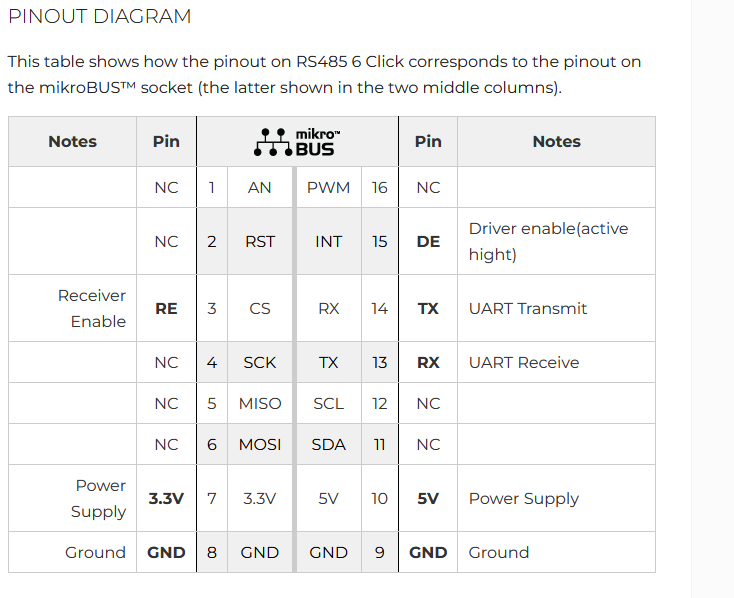
\includegraphics[width=0.5\linewidth]{rs485-pod.png}
    \caption{RS485-6 Pinout Diagram Source: https://www.mikroe.com/rs485-6-click}
    \label{fig:enter-label}
\end{figure}
\begin{figure}
    \centering
    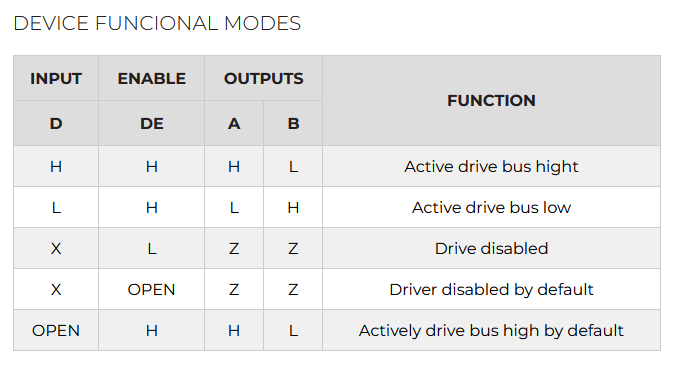
\includegraphics[width=0.5\linewidth]{rs485-dfm.png}
    \caption{RS485-6 Device Funcional Modes: https://www.mikroe.com/rs485-6-click}
    \label{fig:enter-label}
\end{figure}
\subsubsection{RS485-6-Click references}
\url{https://www.mikroe.com/rs485-6-click}
\url{https://libstock.mikroe.com/projects/view/3207/rs485-6-click}